Onto day two! Today I'll again be at the Doctoral Consortium.


\subsection{Sandhya Saisuramanian: Adaptive Modeling for Risk-Aware Decision Making}

Agents: commonly use ``reduced models" -- a simplified model of the world. \\

Simplified for: 1) tractability, 2) unavailable information. \\

To simplify the world, we could change the {\it state} space or the {\it action} space -- in this work, we'll focus on restricting the action outcomes. \\

Drawbacks of planning with reduced models:
\begin{enumerate}
    \item Over optimistic
    \item Sub-optimal action selection
    \item Excessive replanning
    \item Unreachable goal(s) from some/all states
\end{enumerate}

Reduced model literature: Improving Planning time (FF, FF-replan)~\cite{yoon2007ff}, bounded number of exceptions~\cite{pineda2014planning}. \\

Q: How do we choose the right reduced model? \\

A: it's hard! 1) Representation is problem specific, 2) trade-off in simplicity/risk, 3) Hard to deal with incomplete information. \\

{\bf Thesis:} Investigate how to improve risk awareness by taking into account the complexity of planning under uncertainty. \\

Current Focus:
\begin{enumerate}
    \item Improving model fidelity to address over optimism
    
    $\ra$ Main Idea: selectively improve model fidelity by accounting for risky outcomes in selected states. Do so by setting a threshold based on amortizing risk.
    
    \item Replanning in critical states
\end{enumerate}

One idea: ``determinize" $(s,a)$ pairs by ignoring some of their stochastic outcomes. This leads to a simpler model. Conduct experiments showing the impact of different thresholds on when to determinize, showing a decrease in risk. \\

In the future, hope to extend these ideas to settings with incomplete information. \\

Q: Slide 24: time savings relative to what? \\

Q: Why use this measure for the effectiveness of a reduction? $Q - $.

\spacerule
\subsection{Abhinav Verma: Interpretable and Verifiable RL through Program Synthesis}

Example: a deep RL agent (DDPG) trained a simulation of a car driving. \\

But, we shouldn't actually {\it deploy} this trained agent even it if works in simulation. \\

So, the goal of this work: how can we systematically uncover failures/weaknesses/strengths of the approach? \\

Running Example: The Open Racing Car Simulator (TORCS) -- continuous control task involving driving a race car around a track. Quite complex: high dimensional input, agent controls steering/acceleration/breaks. \\

{\bf Goal:} Change our policy representation to something more interpretable. \\

Q: What does that mean? \\

A: Previously, we use a neural network for a policy. Now, we'll instead propose a programmatic policy. Gives us access to more logical/symbolic kinds of understanding about the agent. \\

{\bf Main Idea:} Automatically discover expressive policies in a high level domain specific language for RL environments. \\

$\ra$ Method is to use DRL to find a good policy and distill it into a high level program. \\

Main Benefits: 1) Interpretability, 2) Verifiability (that is, we can prove properties like robustness),  and 3) Generalizability. \\

Challenge: Searching for a good programmatic policy is hard. The search space is non-smooth, need to do many rounds of discrete optimization. \\

$\ra$ Can address this challenge by defining a domain specific language so that the policy search space is much smaller (so, instead of unleashing a Turing complete language, instead look at task-specific conditions/concepts). \\

To handle the optimization problem, use some imitation learning. \\

Experiment on a transfer variant of the racing domain, find smooth policies (w.r.t. the driving of the car), and good performance on tracks on seen at training time.

\spacerule
\subsection{Ruohan Zhang: Attention -- From Data to Computational Models}

{\bf Goal:} Understand biological attention mechanism at the behavioral and neural level. \\

$\ra$ If we can understand these mechanisms well enough, we can open doors to new techniques in AI/RL. \\

Humans have {\it foveated} vision: full-resolution vision in the central 1-2 visual degree of the field. \\

Neat example of a person playing the Atari game Freeway, showing the gaze of the person dart around the screen as they play. \\

{\bf Research Question 1:} How do we vuild a visual attention model from eye movement data? \\

Collect data-sets of: 1) a person playing some Atari games, 2) a person walking outside on rough terrain with fully body motion capture, 3) virtual data driving in urban areas. \\

Propose a ``Gaze Prediction Network" that takes as input 4 consecutive images and outputs predicted probability distribution of gaze. \\

Results are promising! Predicted distribution matches groun truth well. \\

{\bf Research Question 2:} Can we use insights from attention to do imitation learning more effectively? \\

Simplest form of imitation learning is called ``behavioral cloning", in which the learner tries to exactly match the demonstrator's behavior. \\

Now, the new Q: predict a human player's action given in a game frame. \\

Idea: use the predicted gaze to bias a network in both action prediction (in imitation learning) and in RL. In both cases the gaze helps learning across a variety of Atari games.

\spacerule
\subsection{Faraz Torabi: Imitation Learning from Observation}

Example: Babies playing with each other after watching a Pixar movie (where two characters do the same!). \\

{\bf Research Question:} In what ways can autonomous agents learn to imitate experts using visuals observations? \\

Main Contributions:
\begin{itemize}
    \item A model-based algorithm for imitation from observation
    $\ra$ + An application of the algorithm in sim-to-real transfer
    \item A model-based algorithm for imitation from observation
    $\ra$ + An application of the algorithm in sim-to-real transfer
\end{itemize}

Imitation learning: learn how to make decisions by trying to imitate another agent. \\

Typical assumption: observations of other agent consists of state-action pairs. \\

$\ra$ Challenge: we don't often have state-action pairs! Often we just have observations, not states or actions (action ontology might not be the sae). \\

Approach 1: model based approach. Consider convential imitation learning $D_{train} = \{(s_0, a_0), \ldots\}$. But now: $D_{train} = \{(s_0), \ldots\}$. \\


$\ra$ Algorithm: Behavioral Cloning from Observation (BCO). Run some policy in the environment to learn an inverse dynamics model which is then used to {\it predict} the missing actions from $D_{train}$. \\

Experiments in Mujoco (``Ant"), demonstrator works very well. Traditional imitation learning methods work, but they have access to actions to learn from. Their approach (without actions!) performs competitively. \\

Next Q: Can we do Sim-To-Real transfer with BCO? \\

A: Yep! Great setting for imitation learning since physical robot trajectories are costly to collect, but simulation is cheap. \\


Final approach: model-free! Generative Adversarial Imitation from Observation (GAIfO). Experimental results are promising! Also experiment with a manipulator robot. \\

%Q: in BCO, How do you choose the exploration policy in learning the inverse dynamics model? Exploration? What if state-only demonstrations don't go to that region?
\spacerule
\subsection{Christabel Waylacce: Stochastic Goal Recognition  Design}

Point: most activities are goal oriented. \\

\ddef{Goal Recognition}{The problem of goal recognition involves identifying the goal of a given actor.}

Lots of applications -- security domains! build the environment to identify dangerous actors, intelligent tutors (what is the objective of the student?) and so on. \\

Problem: Goal Recognition Design (GRD). Want to find behavior that communicates the goal of an agent as early as possible. \\

Metric for describing worst-case: ``worst-case distinctiveness" (wcd) -- the longest sequence of actions an agent can take without revealing its goal. Want to find changes to environments that minimizes the wcd. \\

Three Typical Assumptions:
\begin{enumerate}
    \item Agents are optimal
    \item Action outcomes are deterministic
    \item All agents have full observability
\end{enumerate}

But: lots of limitations imposed by these assumptions! \\

{\bf Research Question:} What are the advantages and limitations of relaxing assumptions in the GRD? People are suboptimal! Lots of stochastic action outcomes. And, agents are always under partial observability. \\

Lots of related work that relaxes some of these assumptions, but not all~\cite{keren2015goal}. This work builds on this prior literature by relaxing the determinism assumption. \\

Objective: GRD problem, but now minimize the {\it expected case distinctiveness}. Also extend this to {\it partially observable} case, where now actions can be stochastic and we only receive observables, not states.

\spacerule
\subsection{Satyha Ravi: Numerical Optimization to AI and Back}

Consider Regularization: some method we have for preventing our learning algorithms from overfitting:
\begin{itemize}
    \item Explicit Regularization: Constraints, penalties.
    \item Implicit Regularization: algorithms, priors.
\end{itemize}

This work: mostly focused on the use of {\it constraints}:

$\ra$ Experimental design for sparse models: well studied when function of interest is linear (can be solved with convex optimization).

Problem: $D$-Optimal design, with resource constraints:
\[
\min_{S \subset N} \log \det \left(\sum_{i \in S} x_i x_i^T\right)^{-1}, \hspace{6mm} \text{s.t. } |S| \leq B.
\]

Can translate the above into a convex optimization problem. \dnote{(I missed the details of what the variables above denote)}. Evaluate on a Neuroimaging dataset. \\

Next: flow problem -- that is, given two images, track something about the movement of pixels between the images. Goal is to develop general purpose algorithm for all sorts of flow problems. 
\spacerule
\subsection{Atena Tabakhi: Preference Elicitation for Constraint-Based Methods}

Example: Smart Home Device Scheduling (SHDS). We'd like our home to automatically infer our preferences about how to manage aspects of our home (lights, temperature, etc.). \\

{\bf Objective:} find a schedule that minimizes power consumption and discomfort of homeowners. \\

Induces a Weighted Constraint Satisfication Problem (WCSP):
\ddef{WCSP}{$P = <X,D,F>$:
\begin{itemize}
    \item $X$ set of variables
    \item $D$ set of finite domains for each variable
    \item $F$ set of constraints, assigns a cost to each constraint.
\end{itemize}
Solution: an optimal assignment $\vec{x}$ that minimizes the sum over all costs.}


{\bf Research Method 1:} Interleaving search and elicitation. \\

First approach: use a brute force approach (BFS) to find assignments. Then, propose 3 parameterized heuristics: 1) Least Uknown Cost Elicitation (LUC), 2) Least Known Cost Elicitation (LKC), and 3) Combination (COM). \\

Evaluate heuristics empirically, measuring runtimes and costs averaged over 100 random graphs. \\

{\bf Research Method 2:} Preference Elicitation in Preprocessing. \\

Now, modeled as a multi-agent system (multiple owners in same household). Again model this as a WCSP. \\

Two proposed methods for eliciting before solving the problem: Minimax regret (MR) and Maximum Standard Deviation (MS). \\

Further empirical evaluation to evaluate heuristics: 10 homes with 10 devices, time horizon of 6, average over 100 synthetically generated homes. Compare the heuristics vs. the random base-line (RD). \\

Future work: learn user preferences from imperfect feedback or uncertain user feedback.

\spacerule
\subsection{Emmanuel Johnson: Using Automated Agents to Teach Negotiation}

Example: Intelligent Tutoring System. AI is good at teaching ``hard" skills like math/computing. But! They aren't as effective for``softer" skills like negotiation. \\

In fact: most of us are bad at negotiating. 90\% court cases are settled outside of court through negotiation~\cite{eisenberg2009settlement}. Also important for negotiating salaries. \\

``Negotiation" here means the following: two people, each have a set of preferences over a set of objects. There's a way they can divide these items given these preferences. \\

Import distinction between value claiming and creating:
\begin{itemize}
    \item {\it Value Creating}: the process of maximizing joint utility often referred to as ``growing the pie".
    \item {\it Value Claiming}: the process of getting as much in the negotiation as possible.
\end{itemize}

%Negotiation is rarely taught (just in business/law school).
This work: focused on providing personalized pedagogical feedback to help individuals improve negotiating. \\

Different negotiation principles fit nicely into value creating/claiming buckets, like not committing too early, holding ground, and so on. \\

Data set: conflict resolution agent tests. 156 human-agent negotiations (wizard of oz style -- someone controlling the agent). There's a collection of objects on a table, the person and the bot negotiate back and forth over who gets what objects (video demo: it was awesome!). \\

Metrics: look at predicted outcomes of the deal based on the negotiation principles. Principles measured: good initial claim, agreement time, etc. \\

{\bf Pilot Study:} with the wizard of Oz agent. Study the predicted quality of the negotiation, the amount of information you've gathered from the questions asked, and so on. \\

Main Question: can we get people to claim more value in initial offer and in overall negotiation? \\

Now, move on to a fully automated agent with IAGO~\cite{mell2016iago}. Tested 90 people split into 3 categories: 1) no feedback, 2) general feedback, and 3) personalized feedback. \\

Results: we're good at teaching value claiming, but not value creation. \\

Next steps: maybe we need to rethink how we're capturing value creation. Could draw on opponent model to better understand negotiation. \\

\subsection{Thayne Walker: Multi-Agent Pathfinding in Complex Domains}

Example: would you want to ride in a particular air taxi? \\

Three kinds of taxis: 1) bounded suoptimal, 2) resolution suboptimal, 3) one that replans conveniently around a hot airballoon, and 4) a taxi that moves smoothly around obstacles. \\

So: we want a taxi that can plan quickly and come up with a good solution. \\

{\bf Objective:} Multi-agent planning algorithms that are efficient and have bounded sub-optimality. \\

Classic Multi-Agent Path Finding (MAPF) problem: 

\ddef{Multi-Agent Path Finding}{Consider $k$ agents, each with a unique goal $g_1, \ldots, g_k$, moving in a grid. Agents collide if they move into the same cell. \\

Find the multi-agent policy $\pi : \mc{S} \ra \mc{A}^k$ that delivers all agents to their goals as quickly as possible.}

``Complex Domain" means non-unit costs, variable length action durations, agents with definite size and shape, and movement with variable speeds. \\

Q: Lots of measures of success: low variance over time-to-goal, lower the min, lower the avg, etc. \\

\begin{figure}[h!]
    \centering
    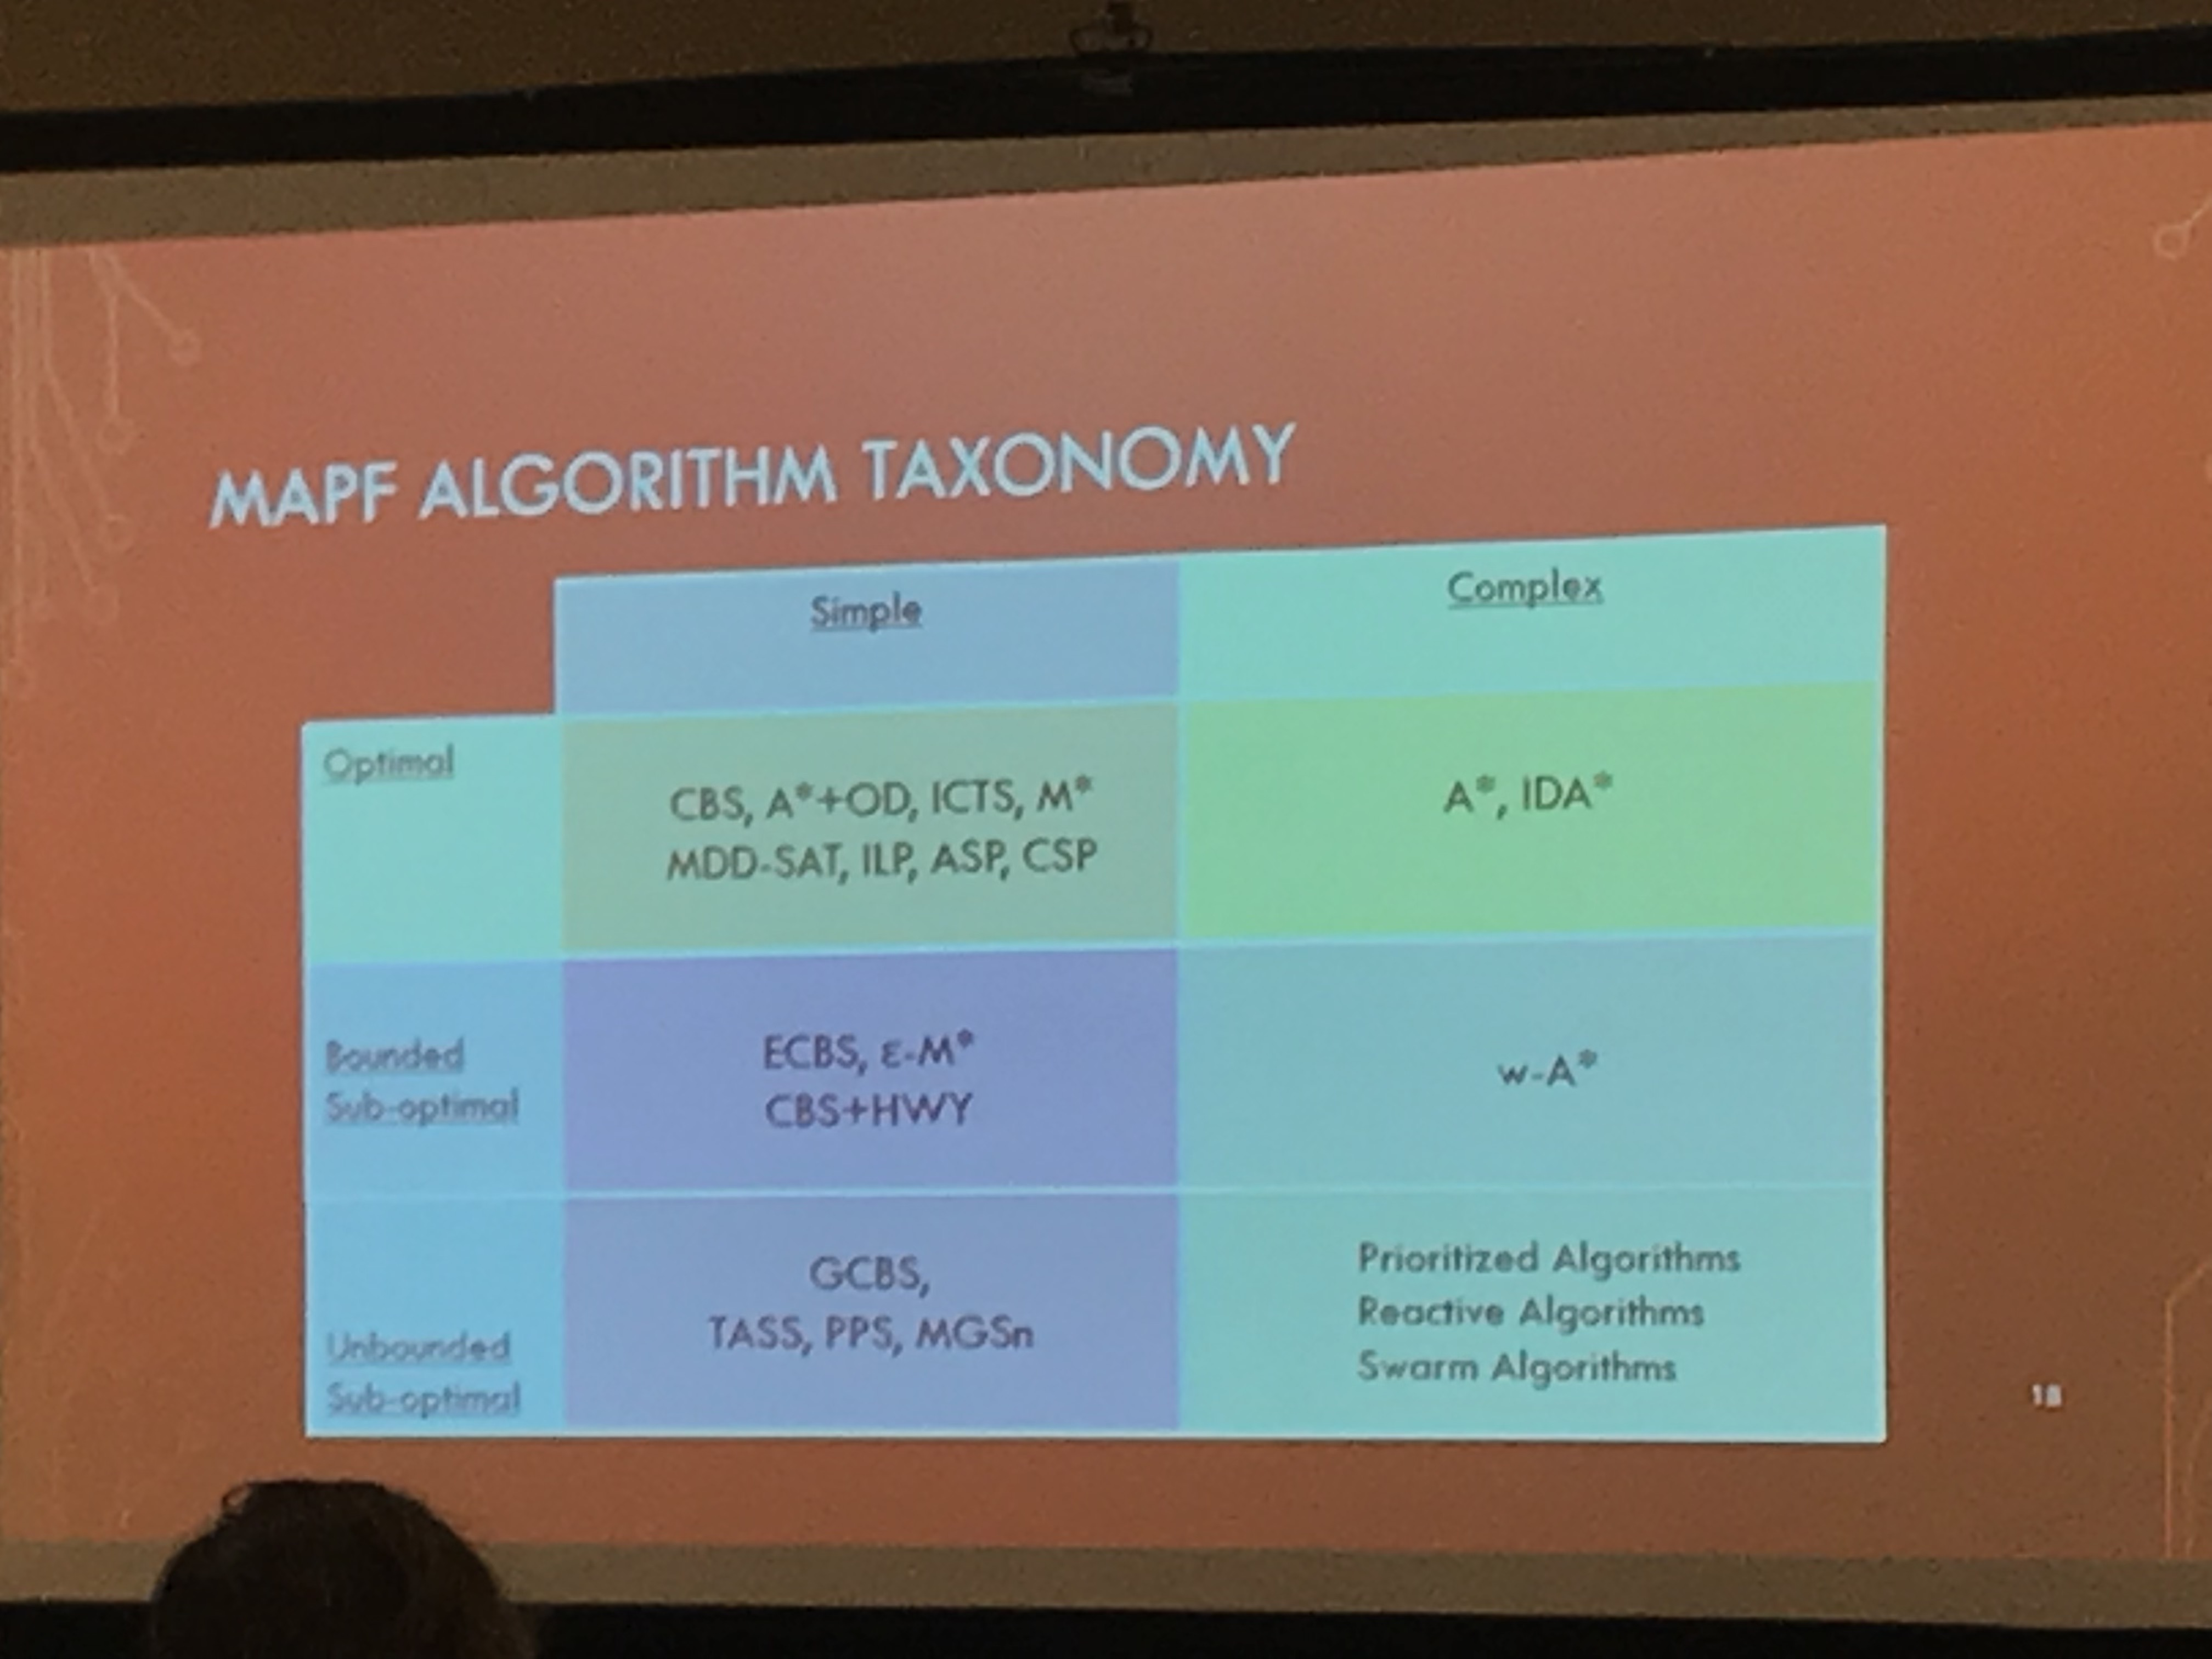
\includegraphics[width=0.5\textwidth]{images/mapf.JPG}
    \caption{Taxonomy of MAPF approaches}
    \label{fig:mapf}
\end{figure}

New approach 1: CBS + CL, which fills in the bottom right slot of Figure~\ref{fig:mapf}. \\

New approach 2: Extended ICTS, which extends the ``increasing cost tree search" algorithm for non-unit costs, which fits in the top right slot of Figure~\ref{fig:mapf}. \\

Current Work: extends conflict based search (CBS) CBS~\cite{sharon2012meta} by adding a conflict avoidance table and prioritization of conflicts. \\

Hypothesis: a particular statistic, ``ecap", can predict the effectiveness of approaches to conflict avoidance. ``ecap" means ``equivalent-cost alternate paths", which is roughly: $\frac{\text{num states in equivalent paths}}{\text{num states in optimal path}}$. \\

Extension: apply constraints over both time, overlaps of paths/edges, and other dimensions/planning constituents.

\spacerule
\subsection{Christopher Fourie: Adaptive Planning with Evidence Based Prediction}

Goal: robot needs to understand what a person is going to do in the context of a joint robot-person collaborative activity. \\

This involves: activity recognition, segmentation, and predictions. \\

Idea: we get less idle time with people/robot if robots can anticipate the person's behavior! So, let's get robots to anticipate behavior. \\

{\bf Research Goal:} Get collaborative systems to accommodate 1) individual behavioral patterns, 2) preferences in task ordering and timing, 3) new behaviors as they occur. \\

Focus: Repetitive Task Environments (RTEs). \\

{\bf Technical Approach:}
\begin{enumerate}
    \item {\it Modeling and an Activity Prediction Framework:} predicting activities in RTEs.
    \item {\it Planning for Improved Fluency:} in RTEs.
    \item {\it Human Experiments:} and the controlled evolution of fluency/efficiency in RTEs.
\end{enumerate}

Human-Study: collect data of people performing a partially ordered task as naturally as possible. Fit a gaussian model to the time taken by each person -- can then evaluate how well that model predicts the time taken for other people. \\

$\ra$ Finding: we're not sure if we can expect models like this to predict orderings and time taken for {\it new} people. Doesn't generalize all that well! Individuals are highly unique. But, inter-ordering behavior is consistent. \\

So, idea: define a temporal predictor for each ordering. Idea is to use a mixture model for predicting time-taken given the ordering (so its a mixture of orderings). \\

Next idea: learn an activity recognition model for sets of trajectories, and use this model to augment the temporal prediction.

\spacerule
% --- AI Roadmap ---
\subsection{AI Roadmap Panel}

To close out the night there will be a panel discussing the next 20 years of AI-research, chaired by Yolanda Gil and Bart Selman. \\

\begin{figure}[h!]
    \centering
    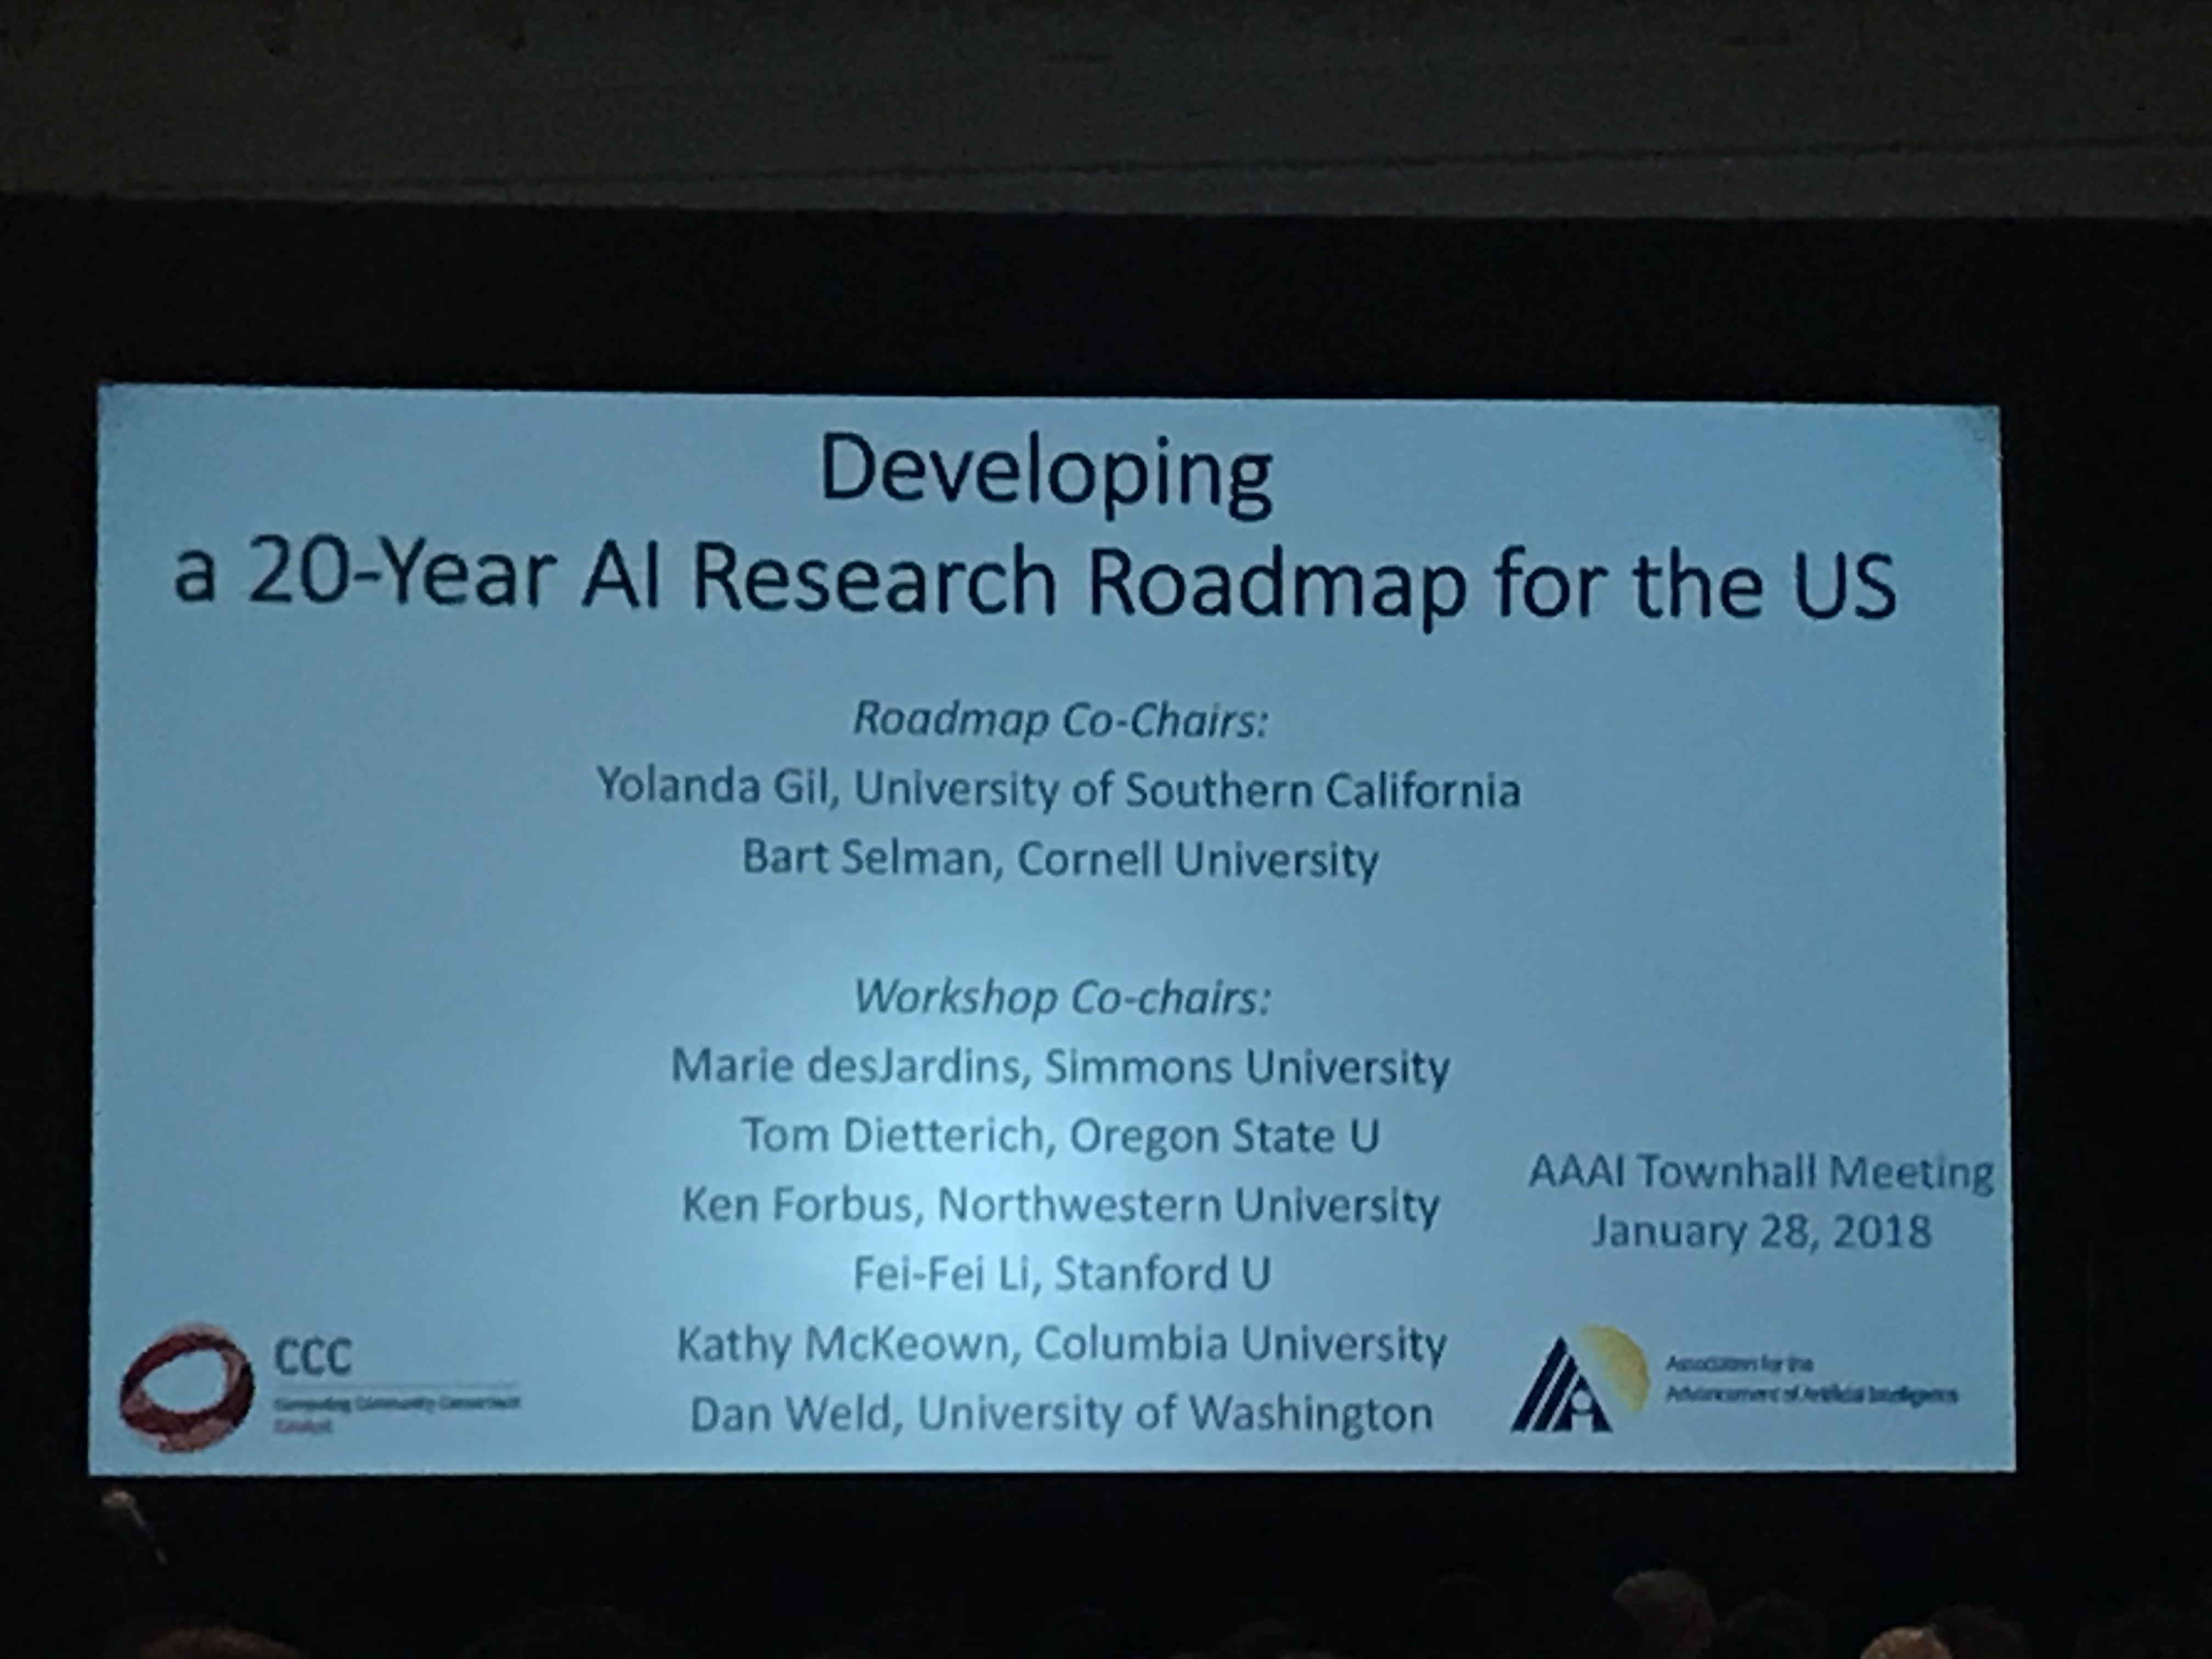
\includegraphics[width=0.5\textwidth]{images/ai_roadmap.JPG}
    \caption{AI Roadmap}
    \label{fig:roadmap}
\end{figure}

US Congress said, in November: we do not want to legislate anytihng about AI/ethics/society, since we (meaning congress) don't understand AI (instead they should turn to researchers). \\

Research roadmap was commissioned by the NSF -- Computing Research Association (CRA) and Computing Community Consortium (CCC) are main institutions behind the roadmap. \\

Objectives:
\begin{itemize}
    \item 10-20 year Roadmap
    \item Guidance for funding agencies and congress.
    \item Relate to AI research in industry.
    \item International AI initiatives.
\end{itemize}

Other documents:
\begin{itemize}
    \item US National AI RandD strategic plan, 2016: \url{https://www.nitrd.gov/news/national_ai_rd_strategic_plan.aspx}
    \item US National Robotics Roadmap, 2006, revised 2006: \url{https://cra.org/ccc/wp-content/uploads/sites/2/2016/11/roadmap3-final-rs-1.pdf}
    \item 100 year study of AI, 2016 report: \url{https://ai100.stanford.edu/}
    \item AI strategies/investments abroad: \url{https://medium.com/politics-ai/an-overview-of-national-ai-strategies-2a70ec6edfd}
\end{itemize}

Held three workshops on 1) Integrated Intelligence, 2) Meaningful Interaction, and 3)

They'll next give summaries of each workshop and their objectives.

\subsubsection{Integrated Intelligence}

Marie Desjardins is the speaker. We thought about three big themes: 1) Mind, 2) Knowledge repositories, and 3) Contextualize AI. \\

{\bf Goal:} Be cross cutting, focus on big interdsciplinary areas that can have big impact. Identified four core areas:
\begin{enumerate}
    \item {\bf Science of integrated AI.} This is all about the {\it integration} of the many subfields we've studied thus far. How do we bring together perception, deliberation, and control? Metareasoning, reflection? What are the components of intelligence?
    \item {\bf Contextualized AI.} involves personalization, social cognition, persistent over time, highly customizable to individuals.
    \item {\bf Open Knowledge Repositories,} we {\it can't} have closed off knowledge bases for individual institutions. This needs to be a community resource! \dnote{Wow that's a fascinating idea.}
    \item {\bf Understanding Human Intelligence.} Unifying theories of human and artificial intelligence, AI to understand human intelligence, and AI inspired by human intelligence.
\end{enumerate}

\subsubsection{Meaningful Interaction}

The speaker is Dan Weld. This workshop focused on collaboration, trust and responsibility, diversity of interaction channels, improving inline interactions. \\

A few societal vignettes to concentrate on, including robot caregivers, training for robot repair jobs, custom personal devices, and so on.

Main technical areas:
\begin{enumerate}
    \item {\bf Collaboration:} how can we model human mental states, get AI systems to understand people better, reliability and ethical behaviors.
    \item {\bf Diversity of Interaction Channels:} diversity of human ability, multimodal explanations, privacy preservation across channels.
    \item {\bf Trust and Responsibility:} Transparency and explanation, debugging behaviors, boundaries and responsibility.
    \item {\bf Improving Interactions Between People:} customized presence, collaborative creation, reputation and factfulness.
\end{enumerate}

\subsubsection{Self-Aware Learning}

The speaker is Tom Dietterich. This workshop focused on robust and trustworthy learning. \\

Main technical areas:
\begin{enumerate}
    \item {\bf Robust and Trustworthy Learning:} Quantifying Uncertainty, identifying risks/failure modes, failing gracefully.
    \item {\bf Deeper Learning for Challenging Tasks:} learning from few examples, learning through interactions, long-term adaption.
    \item {\bf Integration of Symbolic and Numeric Representations:} abstracting symbols from numeric representations, explainable and instructable AI, representing complex structures beyond word embeddings.
    \item {\bf Learning in Integrated AI/Robotic Systems:} robust object manipulation, learning from humans by demonstration and instruction.
\end{enumerate}

\subsection{A New Era of Audacious AI Research}

Now Bart Selman is the speaker. ``Audacious" AI research tackles broader AI goals. Basically: how can we do massive scale AI projects? ({\it a la} the hubble, LHC, human genome project?) \\

Proposed Recommendations:
\begin{enumerate}
    \item {\bf Open National AI Platform:} shared ecosystem/infrastructure for AI research, example resources, data repositories, wide range of contributors, hardware/data/software/services.
    \item {\bf Broaden AI Education:} need for education of official degrees/certifications in AI at all levels, fellowships for grad students, need creative incentive mechanisms.
    \item {\bf Promote AI Policy and Ethics:} promote AI research that focuses on characterizing and quantifying AI systems, need to promote emerging cross-cutting disciplines for AI.
\end{enumerate}


\subsubsection{Q\& A}
Now onto some Q \& A! They also gave out an email address folks can contact with questions or ideas: \url{gil@isi.edu}, \url{selman@cs.cornell.edu}, and \url{cccinfo@cra.org} \\

Q: You mentioned some public resources (like data sets/hardware available for public use) -- who will build such a thing? \\

$\ra$ A: Well, we're mostly defining the agenda, and trying to highlight the landmarks that we can hit if we invest our resources as a society in the right way. \\

Q: If we build a communal knowledge graph, how do we do that in a way that is unbiased? Make it open? Targeted initiatives? \\

$\ra$ A: Yes! We discussed this point a lot. Social norms and counterfactuals and fictional worlds are all very challenging things to embed in a knowledge graph. There will absolutely not be the ``one true" perspective on the world. \\

Q: What's the plan for the roadmap given that governments around the world are realizing the power of AI and are starting to regulate AI? Might interfere with what we do/want to do? \\

$\ra$ A: We take the position that we support fundamental research in AI, and open research in AI. There's a military component that we do not really address. 

$\ra$ A2: many ways folks might want to control AI -- control for good of society, good of individual/country. We discuss control of intellectual property in the doc. Core philosophy: roadmap is how we open the development of AI techniques so we benefit all of society. \\

Q: Sharing info among AI researchers, as with arXiv. Some of the presentations from today were online, for instance. It's helpful to have shared presentations/papers. Any ideas for sharing work more easily? \\

$\ra$ A: That's an important insight! The more we understand each others' expertise/perspective the better. So let's continue to focus on open/accessible software/data/papers. \\

Q: How does modeling business processes show up in the roadmap? \\

$\ra$ A: Definitely came up in the workshop(s). \\

Q: How do companies/industry fit into the roadmap? I didn't see them show up all that much. \\

$\ra$ A: Many folks in industry are involved, lots of people at the workshops were from industry. Your point is well taken and we welcome involvement from industry. \\

\dnote{Now the Q\& A is moving to a more open ``suggestion/general question" session}

Q: A suggestion -- focus on natural disasters (see: Harvey, Katrina, wildfires). \\

Q: Lots of societal challenges on the horizon -- thoughts on how to tackle them? \\

$\ra$ A: well, we're trying to draw on many disciplines to better understand and prepare for this impact. \\

Q: This is really an international problem -- we're working on the same thing in Europe. So, perhaps we should connect our agendas. \\

$\ra$ A: Absolutely! We hope we can work on that soon. \\

Q (from Ed Feignenbaum!): To do what you laid out is going to take an {\it army} of AI research superstars. Half the trickle of people we train go off to Google/Microsoft/Facebook. Are you worried about this education problem? We need an army, we're getting a platoon! \\

$\ra$ A: Yes, this came up. We have to make academia an environment for doing this kind of audacious AI research. People find industry exciting because of the money, people, and research. Great question -- we'll raise this question in the report and will try our best to address this. \\

$\ra$ A2: we had a big discussion about this. Someone {\it during} the workshop got a 7 figure offer. No, we can't match that. But, maybe we can offer something else. \\

$\ra$ A3: Another thing we're addressing is how fast society can adapt to changes of all sorts. Also critical to ensure we can increase the diversity of CS education! \\

Q (CTO of lincoln labs): Aloha! Thanks for hosting this in Hawaii. Reminded of the early days of the internet/digital age: Optimism was huge, but later we found massive issues we didn't predict. My feedback is this: you have an opportunity/responsibility to put forward that perspective. It needs to be at the forefront. \\

Q: Curious about the definition of advancement of AI? What does it mean to progress AI? \\

$\ra$ A: We interpret intelligence very broadly -- human/biological/animal/artificial are all included. \\





Q: Lots of wonderful ideas for areas to focus on -- do you have suggestions for how to improve our research methods going forward, given the demands placed on us as a community?

%Q: Any thoughts on how we can change the incentive structures in the world to encourage the right kinds of work?

Q: So many of us probably saw Mark Zuckerberg explain really basic aspects of facebook and the internet to a panel of senators. My question is: how should we deal with the fact that policy makers will be forced to wrestle with areas they have no expertise in? What can we do to both work effectively with policy makers and make sure knowledgable people are involved in critical decision making?